% ============================================================
%  实验报告（第 3 周）— 王本熙 (25020007117)
%  编译方式: xelatex report3.tex (运行两遍以解析交叉引用)
% ============================================================
\documentclass[a4paper,11pt]{ctexart}

% ---------- 页面布局 ----------
\usepackage[
  top=2.5cm, bottom=2.5cm, left=2.5cm, right=2.5cm,
  headheight=15pt, headsep=0.5cm, footskip=0.8cm
]{geometry}

% ---------- 数学与表格 ----------
\usepackage{amsmath, amssymb}
\usepackage{booktabs}
\usepackage{array}
\usepackage{multirow}

% ---------- 图形与链接 ----------
\usepackage{graphicx}
\usepackage{subcaption}
\usepackage[
  colorlinks=true, linkcolor=blue!70!black,
  citecolor=blue!70!black, urlcolor=teal!80!black
]{hyperref}
\usepackage{xcolor}

% ---------- 代码块 ----------
\usepackage{listings}
\definecolor{codebg}{RGB}{248,248,248}
\definecolor{codekw}{RGB}{0,0,180}
\definecolor{codecmt}{RGB}{0,128,0}
\definecolor{codestr}{RGB}{180,0,0}
\lstset{
  backgroundcolor=\color{codebg},
  basicstyle=\ttfamily\small,
  keywordstyle=\color{codekw}\bfseries,
  commentstyle=\color{codecmt},
  stringstyle=\color{codestr},
  numbers=left, numberstyle=\tiny\color{gray},
  frame=single, rulecolor=\color{gray!40},
  breaklines=true, showstringspaces=false,
  tabsize=2, columns=flexible,
  language=python
}

% ---------- 页眉页脚 ----------
\usepackage{fancyhdr}
\pagestyle{fancy}
\fancyhf{}
\fancyhead[L]{\small 王本熙 \quad 25020007117}
\fancyhead[R]{\small 实验报告（第 3 周）}
\fancyfoot[C]{\thepage}
\renewcommand{\headrulewidth}{0.4pt}

% ---------- 章节标题样式 ----------
\usepackage{titlesec}
\definecolor{secblue}{RGB}{30,80,160}
\titleformat{\section}
  {\Large\bfseries\color{secblue}}{第\thesection\,章}{0.6em}{}
\titleformat{\subsection}
  {\large\bfseries\color{secblue!80!black}}{\thesubsection}{0.5em}{}
\titleformat{\subsubsection}
  {\normalsize\bfseries\color{secblue!60!black}}{\thesubsubsection}{0.5em}{}

% ---------- 超链接元信息 ----------
\hypersetup{
  pdftitle={系统开发工具基础实验报告（第 3 周）},
  pdfauthor={王本熙}
}

% ============================================================
\begin{document}

% ---------- 封面 ----------
\begin{titlepage}
  \centering
  \vspace*{2cm}
  {\Huge\bfseries\color{secblue} 实验报告\par}
  \vspace{0.5cm}
  {\Large 系统开发工具基础 \quad 第 3 周\par}
  \vspace{3cm}
  \begin{tabular}{rl}
    \Large 姓\quad 名\,:\, & \Large 王本熙 \\[0.8em]
    \Large 学\quad 号\,:\, & \Large 25020007117 \\[0.8em]
    \Large 日\quad 期\,:\, & \Large 2026 年 9 月 7 日 \\[0.8em]
    \Large 平\quad 台\,:\, & \Large Windows + WSL (Ubuntu) \\
  \end{tabular}
  \vfill
  \rule{10cm}{0.4pt}
  \vspace*{1cm}
\end{titlepage}

% ---------- 目录 ----------
\tableofcontents
\newpage

% ============================================================
\section{实验目的}

本实验旨在掌握以下内容：
\begin{itemize}
  \item 从源码构建 Python 命令行包并在干净虚拟环境中通过 wheel 安装（q09）；
  \item 让编程智能体进入可验证的测试驱动修复循环：先写失败测试，再让智能体修改实现并通过（q10）；
  \item 将"无法处理"的协作材料改写为可执行信息：Issue、提交信息、评审意见的专业写法（q11）；
  \item 补全 PyTorch 线性回归训练循环：\texttt{zero\_grad}/\texttt{backward}/\texttt{step}、\texttt{eval}/\texttt{no\_grad}
        评估模式，最终损失应小于 0.001（q12）。
\end{itemize}

% ============================================================
\section{实验环境}

\begin{table}[htbp]
  \centering
  \caption{实验环境}\label{tab:env}
  \begin{tabular}{ll}
    \toprule
    项目 & 配置 \\
    \midrule
    操作系统 & Windows + WSL (Ubuntu 24.04) \\
    Shell & bash \\
    Python & 3.12.3 \\
    编辑器 & VS Code / Trae IDE / micro \\
    版本管理 & Git \\
    远程仓库 & GitHub \\
    PyTorch & 2.1.0+cpu \\
    \bottomrule
  \end{tabular}
\end{table}

% ============================================================
\section{q09：从源码构建并在干净环境安装 Wheel}

\subsection{题目要求}

主题：Packaging and Shipping Code。创建一个最小 Python 命令行包，并验证 wheel 安装：
\begin{itemize}
  \item 创建 \texttt{src/greetlab/\_\_init\_\_.py}、给定的 \texttt{cli.py} 和 \texttt{pyproject.toml}，
        把"学号"替换为自己的学号 \texttt{25020007117}；
  \item 在已安装 build 工具的课程环境中运行 \texttt{python -m build}，生成 wheel；
  \item 新建一个干净虚拟环境，只从生成的 wheel 安装；
  \item 切换到 q09 之外运行 \texttt{sdt-greet --name <学号>}，确认输出正确。
\end{itemize}

\subsection{实验步骤}

按题目给定内容创建三个文件（\texttt{pyproject.toml} 中学号已替换为 \texttt{25020007117}）：

\begin{lstlisting}[language=Python]
# src/greetlab/__init__.py
# 空文件，标记目录为 Python 包

# src/greetlab/cli.py
import argparse

def main():
    p = argparse.ArgumentParser()
    p.add_argument("--name", required=True)
    a = p.parse_args()
    print(f"Hello, {a.name}!")
\end{lstlisting}

\begin{lstlisting}[language=bash]
[build-system]
requires = ["setuptools>=68"]
build-backend = "setuptools.build_meta"

[project]
name = "greetlab-25020007117"
version = "0.1.0"

[project.scripts]
sdt-greet = "greetlab.cli:main"

[tool.setuptools.packages.find]
where = ["src"]
\end{lstlisting}

随后在 WSL 终端中依次执行：

\begin{lstlisting}[language=bash]
mkdir -p q09/src/greetlab
micro q09/src/greetlab/__init__.py   # 空文件
micro q09/src/greetlab/cli.py        # 写入 main()
micro q09/pyproject.toml             # 替换学号

cd q09
python3 -m venv venv
source venv/bin/activate
pip install build -i https://pypi.tuna.tsinghua.edu.cn/simple

python -m build          # 生成 dist/greetlab_25020007117-0.1.0-py3-none-any.whl
\end{lstlisting}

构建成功后，创建干净虚拟环境验证 wheel 安装：

\begin{lstlisting}[language=bash]
cd ~
python3 -m venv venv_clean
source venv_clean/bin/activate
pip install ~/q09/dist/greetlab_25020007117-0.1.0-py3-none-any.whl

sdt-greet --name 25020007117   # 输出: Hello, 25020007117!
\end{lstlisting}

\subsection{运行结果与截图}

图~\ref{fig:q09} 记录了从创建包结构、\texttt{python -m build} 构建到干净环境验证的全过程。

\begin{figure}[htbp]
  \centering
  \begin{subfigure}[b]{0.98\textwidth}
    \centering
    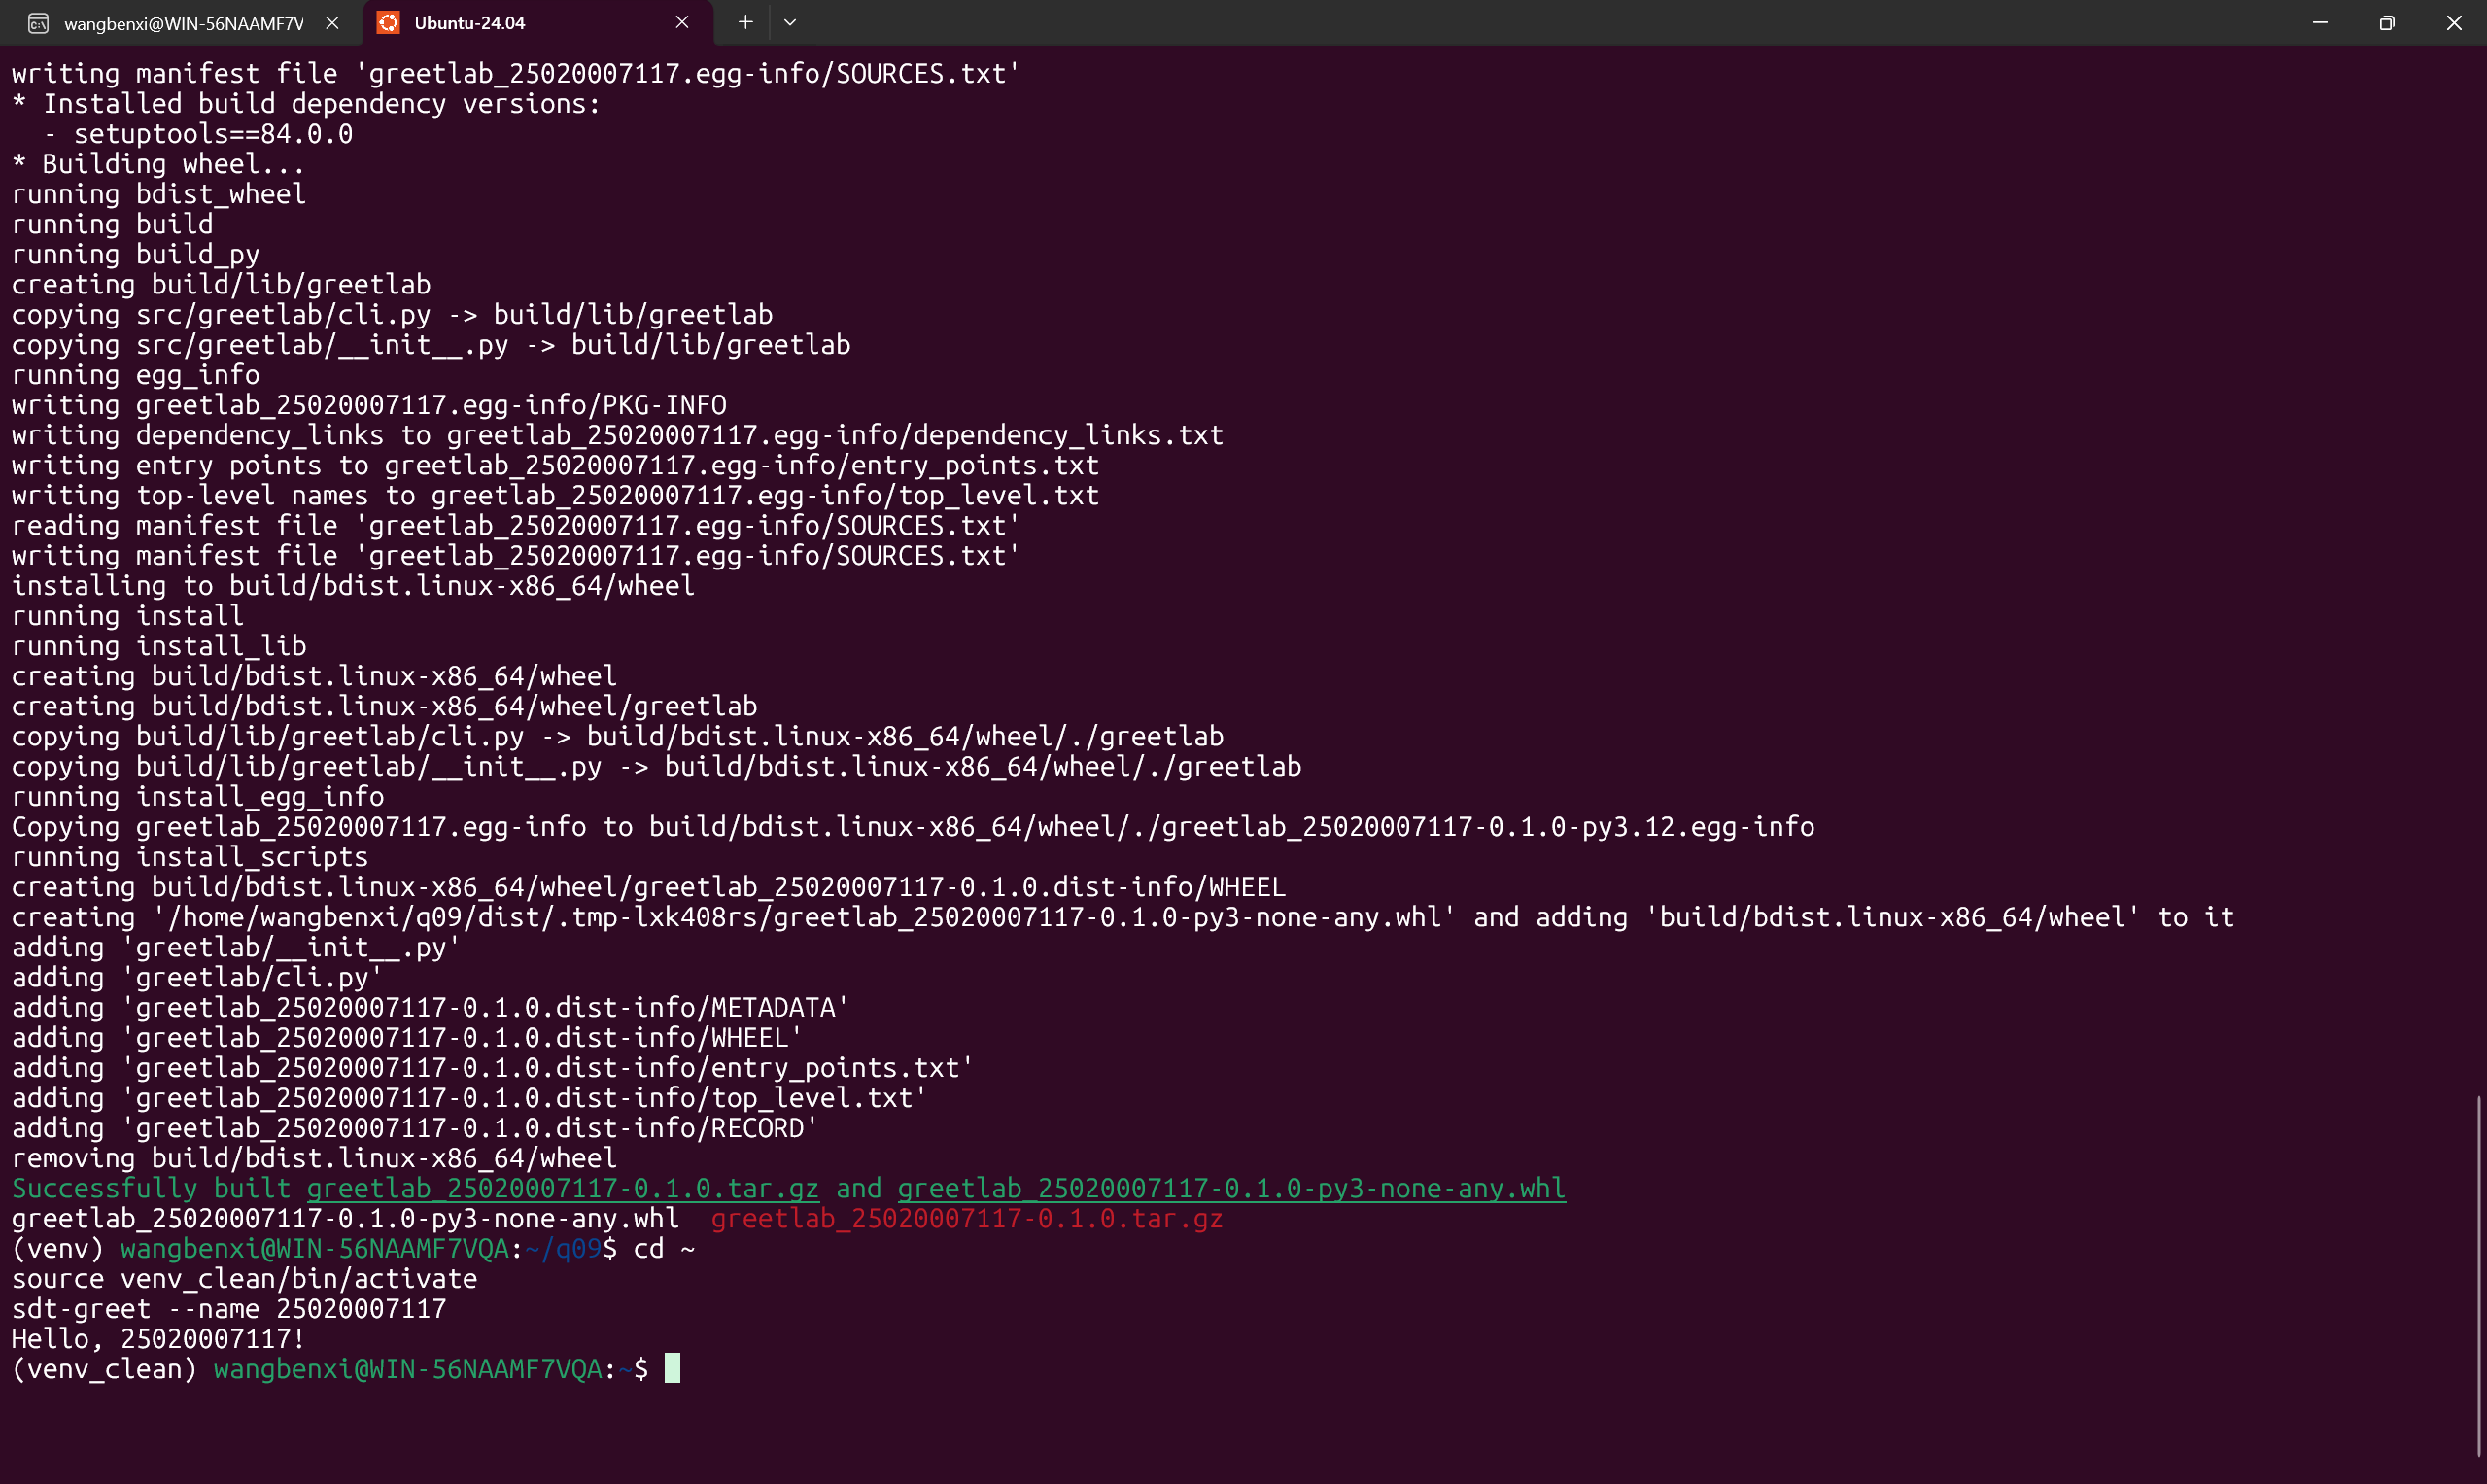
\includegraphics[width=\linewidth]{q09-1.png}
    \caption{创建 \texttt{src/greetlab/} 包结构、\texttt{pyproject.toml}、venv、\texttt{pip install build}、\texttt{python -m build} 构建 sdist 与 wheel}
  \end{subfigure}

  \vspace{0.5em}
  \begin{subfigure}[b]{0.98\textwidth}
    \centering
    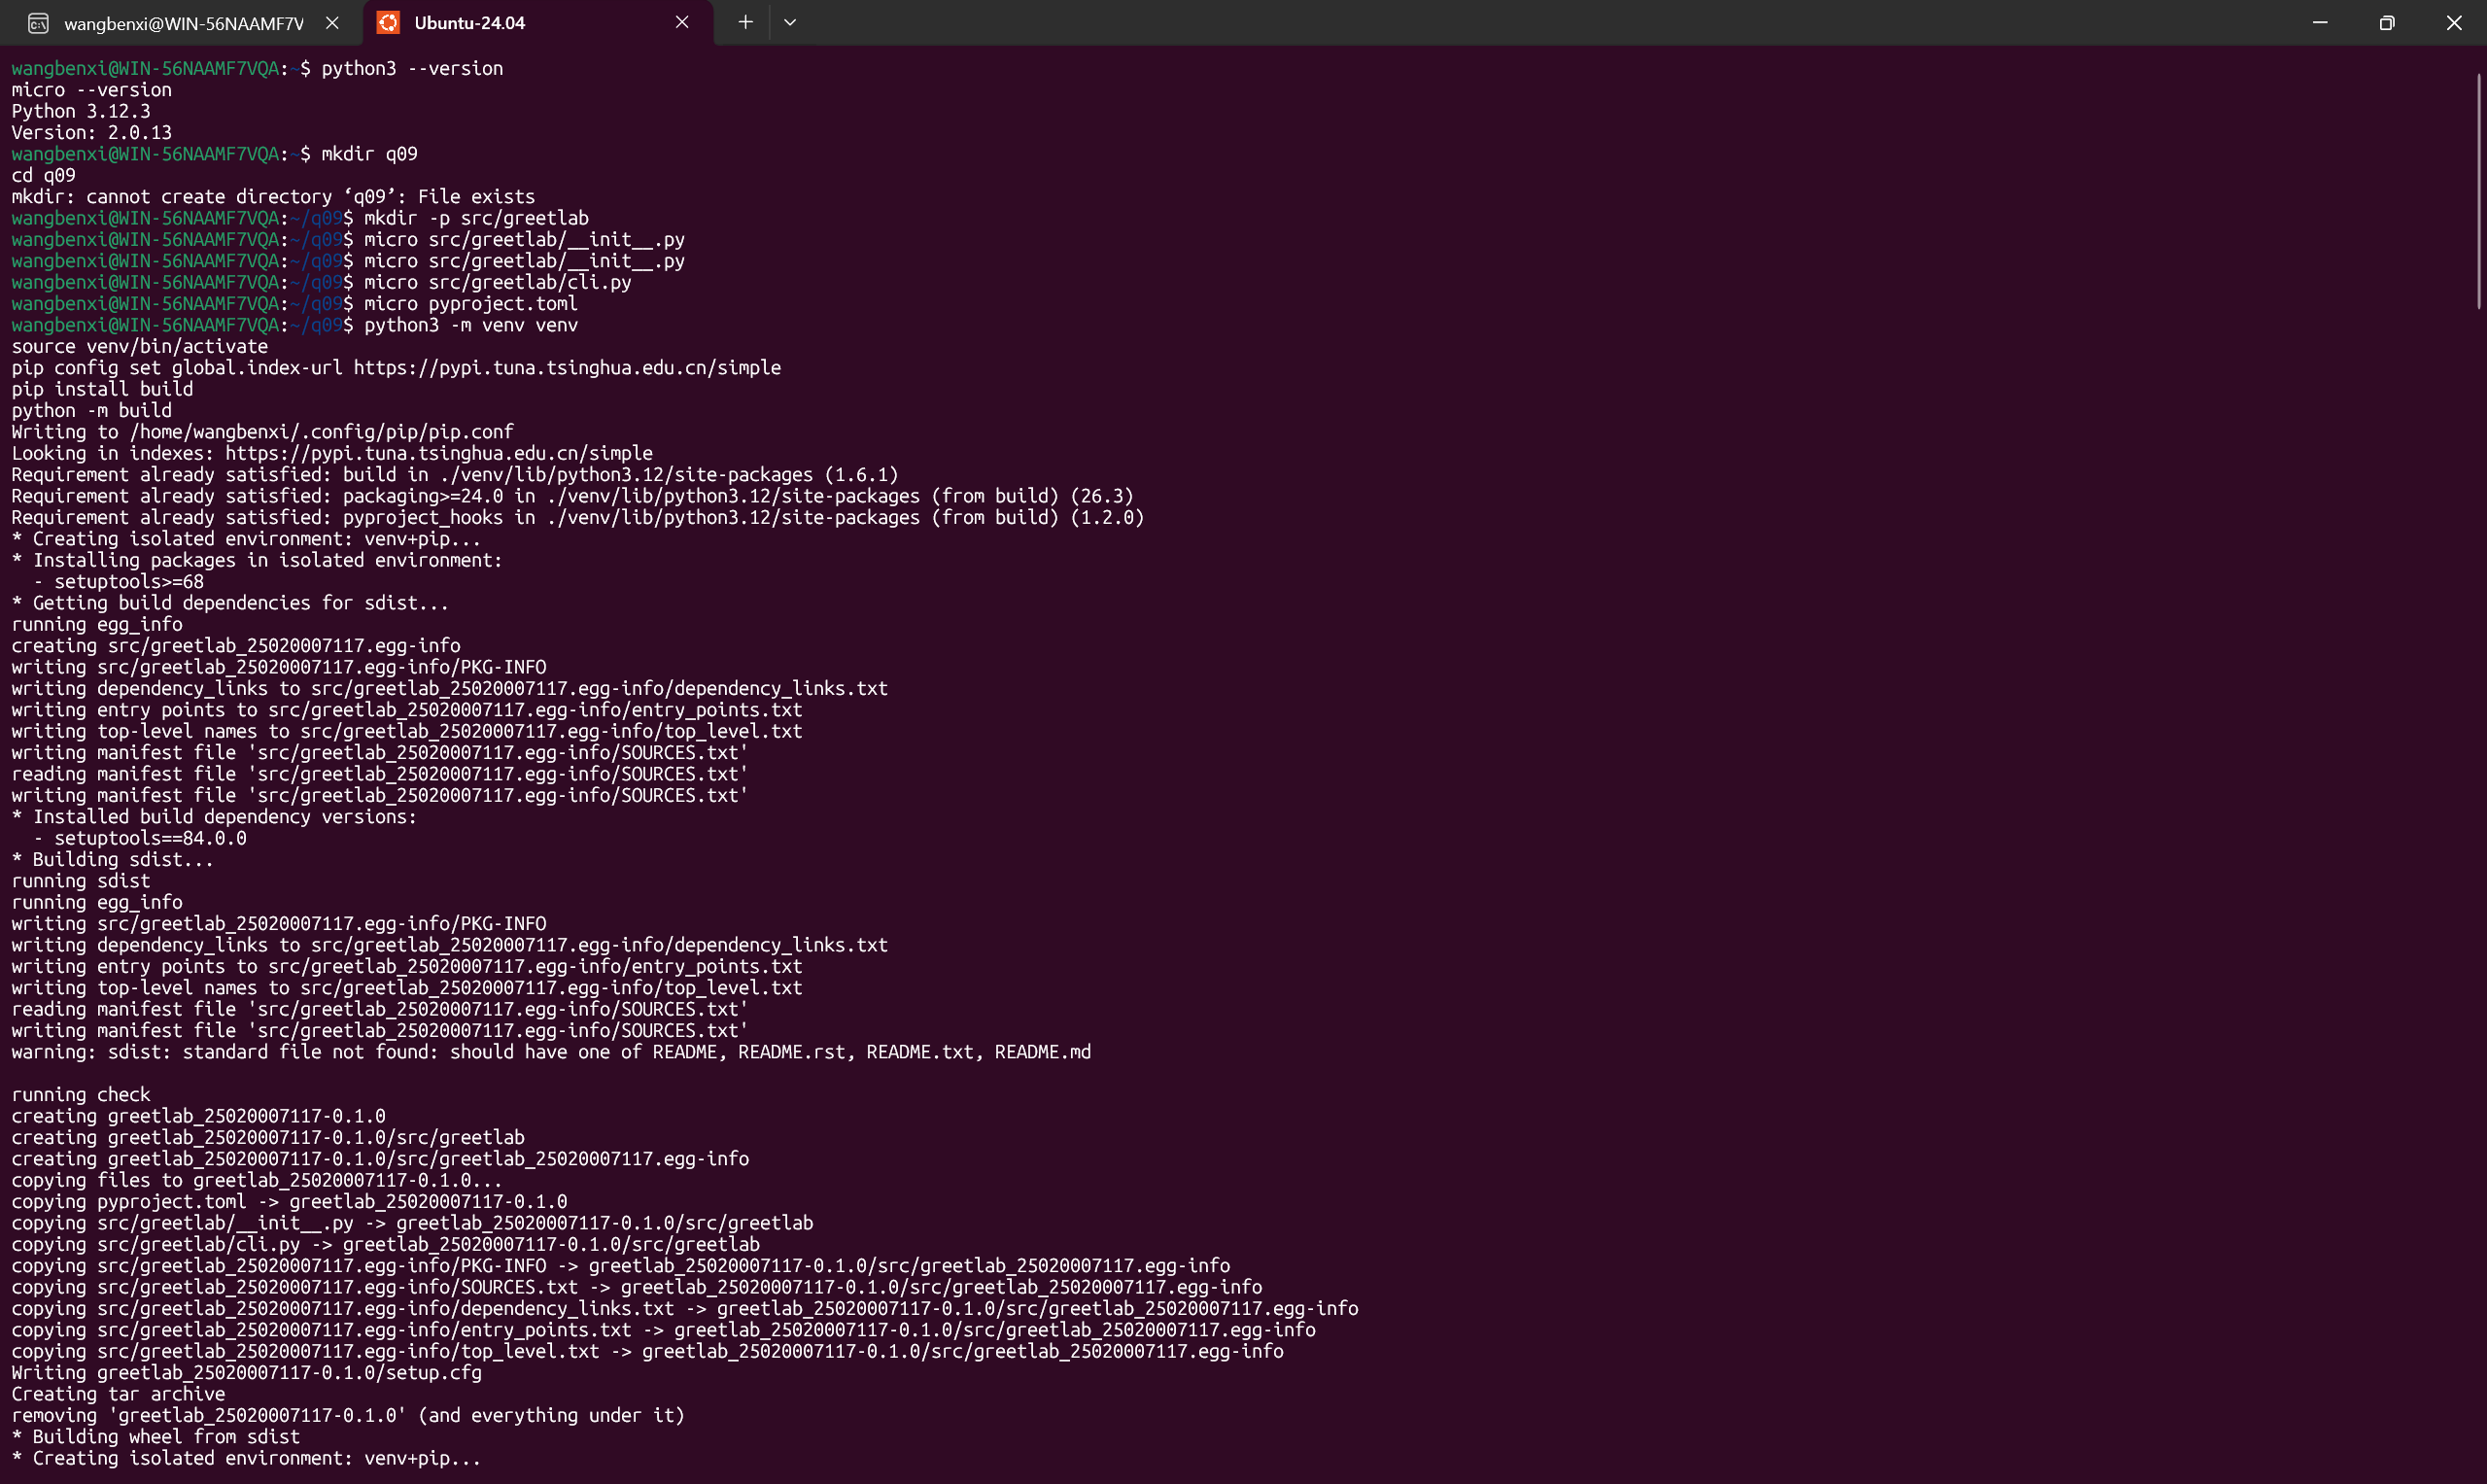
\includegraphics[width=\linewidth]{q09-2.png}
    \caption{\texttt{Successfully built greetlab\_25020007117-0.1.0-py3-none-any.whl}，干净环境安装后 \texttt{sdt-greet --name 25020007117} 输出正确}
  \end{subfigure}
  \caption{q09：从源码构建 wheel 并在干净环境安装验证}
  \label{fig:q09}
\end{figure}

\subsection{结果分析}

\begin{itemize}
  \item \textbf{包结构与 \texttt{pyproject.toml}}：使用 src-layout（\texttt{src/greetlab/}），
        \texttt{pyproject.toml} 配置 \texttt{[project.scripts]} 定义入口点
        \texttt{sdt-greet = "greetlab.cli:main"}，\texttt{[tool.setuptools.packages.find]} 指定
        \texttt{where = ["src"]}，保证构建时能正确找到包；
  \item \textbf{\texttt{python -m build}}：该工具自动创建隔离的构建环境，依次运行
        \texttt{sdist} 和 \texttt{bdist\_wheel}，生成 \texttt{dist/} 目录下的
        \texttt{.tar.gz} 和 \texttt{.whl}；日志中
        \texttt{Successfully built greetlab\_25020007117-0.1.0-py3-none-any.whl} 确认构建成功；
  \item \textbf{干净环境验证}：\texttt{venv\_clean} 不依赖源码、不安装 pytest/ruff，
        仅从 wheel 安装包。运行 \texttt{sdt-greet --name 25020007117} 输出
        \texttt{Hello, 25020007117!}，证明 wheel 自包含了所有运行时所需内容，
        入口点正确注册到 \texttt{PATH}；
  \item \textbf{无 README 警告}：构建日志中
        \texttt{warning: sdist: file not found: README, README.rst, README.txt, README.md}
        仅为警告，不影响 wheel 生成——正式项目应在 \texttt{pyproject.toml} 中
        配置 \texttt{[project.readme]} 消除该警告。
\end{itemize}

% ============================================================
\section{q10：让编程智能体进入可验证的修复循环}

\subsection{题目要求}

主题：智能体编程。复用第 9 题的 \texttt{greetlab} 包，使用编程智能体完成一个小型测试驱动修复：
\begin{itemize}
  \item 复制 q09 为 q10，添加一个失败测试：当 \texttt{name} 只含空白字符时，
        \texttt{main} 应以 \texttt{SystemExit(2)} 结束；
  \item 先运行测试确认失败，再向编程智能体说明目标、约束和测试命令，要求它修改实现并运行测试；
  \item 人工检查 diff，撤销无关修改，并再次运行测试；
  \item 在 \texttt{ai\_log.md} 中用不超过 5 行记录核心提示、智能体改动和人工验证。
\end{itemize}

\subsection{实验步骤}

复制 q09 为 q10，添加空白姓名失败测试：

\begin{lstlisting}[language=Python]
# tests/test_cli.py
import sys
import pytest
from greetlab.cli import main

def test_blank_name_raises_system_exit(monkeypatch, capsys):
    monkeypatch.setattr(sys, "argv", ["sdt-greet", "--name", "   "])
    with pytest.raises(SystemExit) as excinfo:
        main()
    assert excinfo.value.code == 2
    captured = capsys.readouterr()
    assert captured.out == ""
\end{lstlisting}

首次运行 pytest 确认失败：

\begin{lstlisting}[language=bash]
cd q10
python -m venv venv && source venv/bin/activate
pip install -e . pytest -i https://pypi.tuna.tsinghua.edu.cn/simple
python -m pytest tests/test_cli.py
# ERROR collecting tests/test_cli.py: ModuleNotFoundError: No module named 'greetlab'
\end{lstlisting}

\texttt{ModuleNotFoundError} 因为未以可编辑模式安装包（\texttt{pip install -e .}），
加上后运行测试：

\begin{lstlisting}[language=bash]
python -m pytest tests/test_cli.py
# 测试失败: main() 对 "   " 不抛 SystemExit
\end{lstlisting}

向智能体发出指令，要求在 \texttt{cli.py} 的 \texttt{main()} 中增加空白校验：

\begin{lstlisting}[language=Python]
# src/greetlab/cli.py (修复后)
import argparse
import sys

def main():
    p = argparse.ArgumentParser()
    p.add_argument("--name", required=True)
    a = p.parse_args()
    if a.name.isspace():
        sys.exit(2)
    print(f"Hello, {a.name}!")
\end{lstlisting}

记录 \texttt{ai\_log.md}：

\begin{lstlisting}
Prompt: 要求智能体在 name 仅含空白时让 main() 以 SystemExit(2) 退出，不改测试文件。
Change: cli.py 增加 isspace() 检查并 sys.exit(2)。
Verify: pytest tests/test_cli.py 通过，diff 仅含 cli.py 一处修改。
\end{lstlisting}

\subsection{运行结果与截图}

图~\ref{fig:q10} 展示了 \texttt{ai\_log.md} 记录、首次 pytest 失败和最终 pytest 通过。

\begin{figure}[htbp]
  \centering
  \begin{subfigure}[b]{0.98\textwidth}
    \centering
    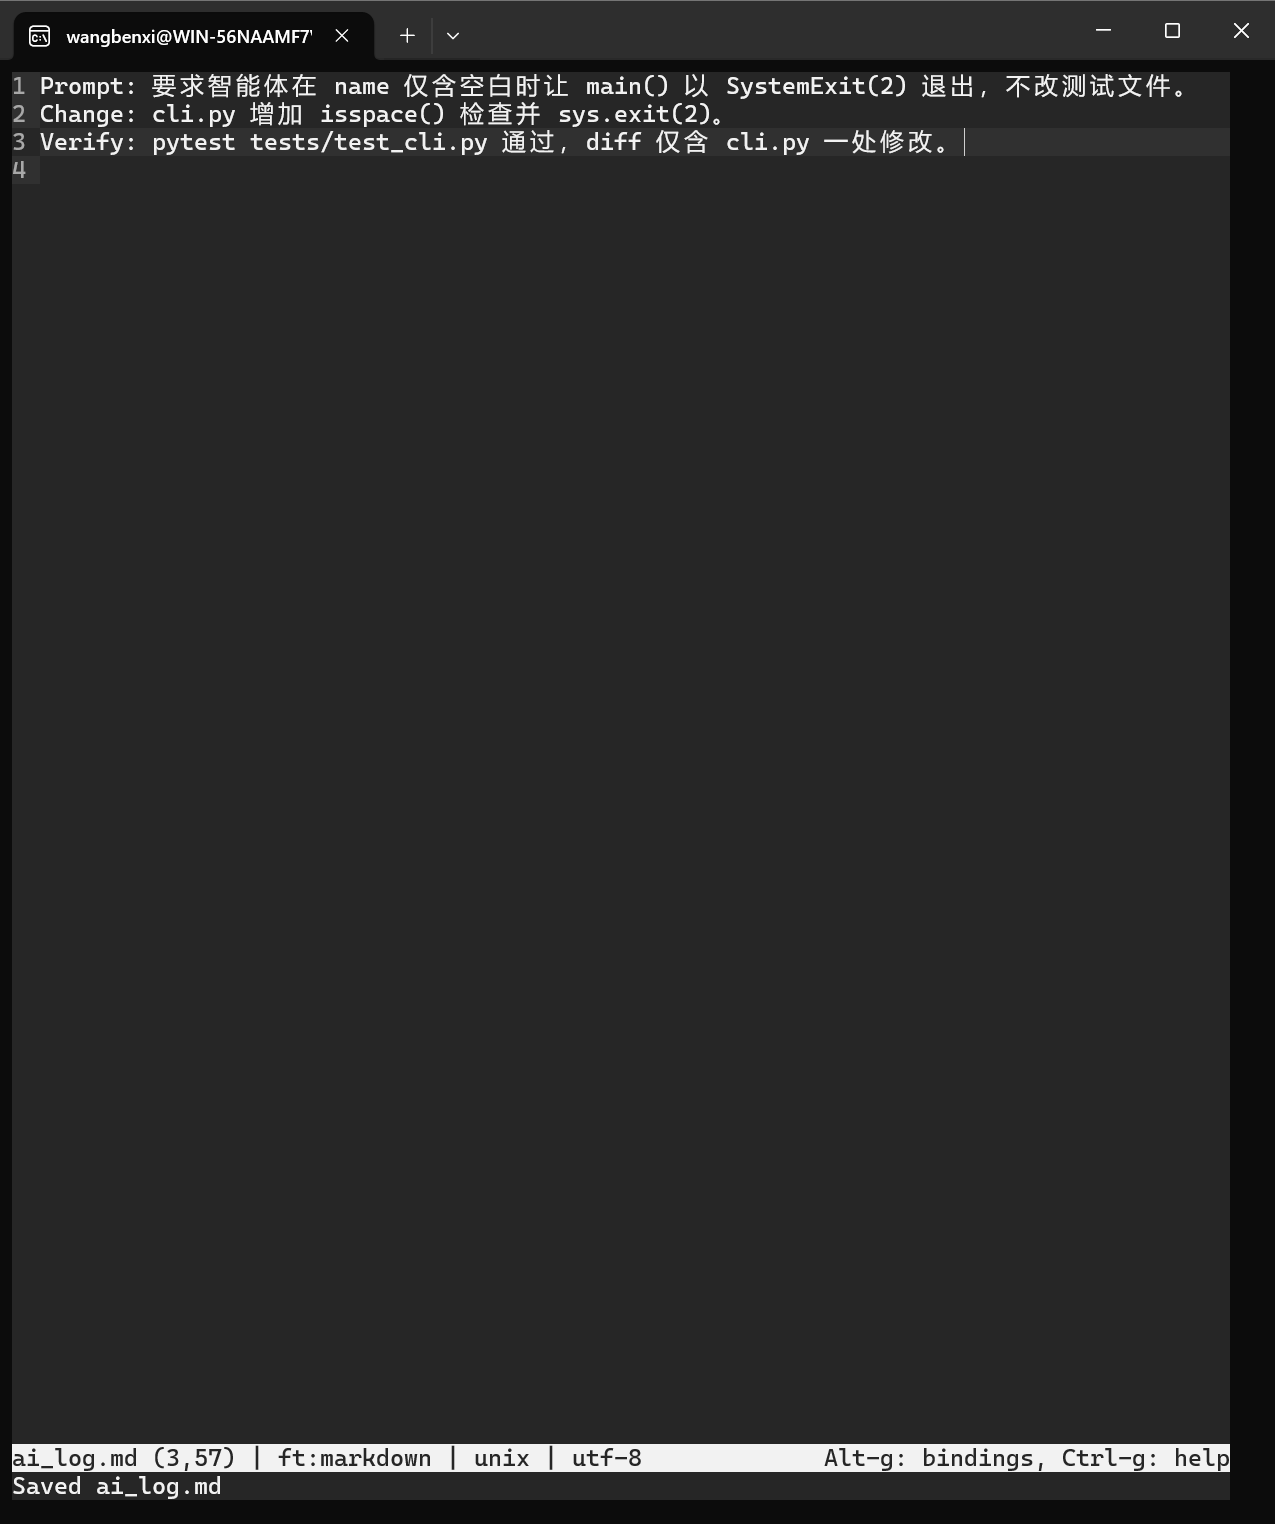
\includegraphics[width=\linewidth]{q10-1.png}
    \caption{\texttt{ai\_log.md}：Prompt / Change / Verify 三行记录智能体交互}
  \end{subfigure}

  \vspace{0.5em}
  \begin{subfigure}[b]{0.98\textwidth}
    \centering
    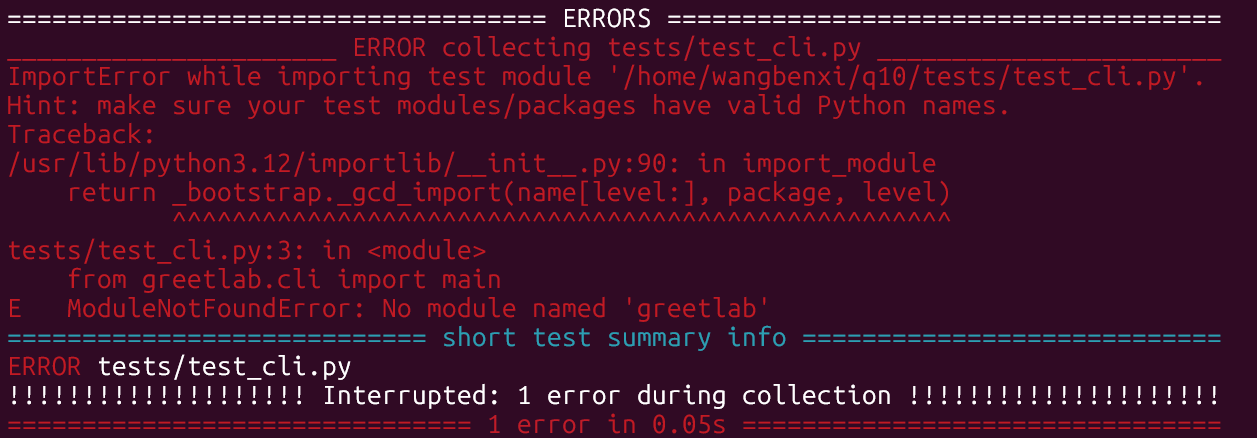
\includegraphics[width=\linewidth]{q10-2.png}
    \caption{pytest 失败：\texttt{ModuleNotFoundError: No module named 'greetlab'}（未以 \texttt{-e} 安装）}
  \end{subfigure}

  \vspace{0.5em}
  \begin{subfigure}[b]{0.98\textwidth}
    \centering
    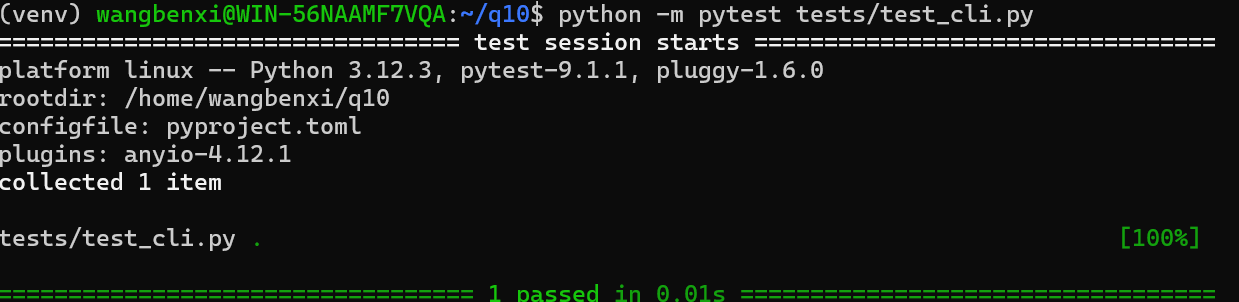
\includegraphics[width=\linewidth]{q10-3.png}
    \caption{\texttt{1 passed in 0.01s}：修复后 pytest 通过}
  \end{subfigure}
  \caption{q10：编程智能体驱动的测试修复循环}
  \label{fig:q10}
\end{figure}

\subsection{结果分析}

\begin{itemize}
  \item \textbf{测试驱动}：先写失败测试 \texttt{test\_blank\_name\_raises\_system\_exit}，
        使用 \texttt{monkeypatch} 注入 \texttt{sys.argv}、
        \texttt{pytest.raises(SystemExit)} 捕获退出码、\texttt{capsys} 捕获 stdout，
        完整模拟命令行参数并验证行为；
  \item \textbf{ModuleNotFoundError 陷阱}：首次运行 pytest 报
        \texttt{No module named 'greetlab'}——因为 \texttt{src-layout} 包需以
        \texttt{pip install -e .} 可编辑模式安装后，pytest 才能在 Python 环境中
        找到 \texttt{greetlab} 包。这是 \texttt{src-layout} 项目调试的常见坑点；
  \item \textbf{智能体修复}：向智能体明确目标（空白 $\to$ SystemExit(2)）、
        约束（不改测试文件）、验证命令（\texttt{pytest tests/test\_cli.py}），
        智能体修改 \texttt{cli.py} 增加 \texttt{isspace()} 检查并调用 \texttt{sys.exit(2)}，
        diff 仅涉及一处修改，无无关改动；
  \item \textbf{ai\_log.md}：用三行记录 Prompt / Change / Verify，
        不超过 5 行，体现了智能体协作中"明确目标 $\to$ 最小修改 $\to$ 可验证"的闭环。
\end{itemize}

% ============================================================
\section{q11：把"无法处理"的协作材料改成可执行信息}

\subsection{题目要求}

主题：不止于代码。围绕"空姓名仍输出问候语"这一缺陷，改写三段质量较差的协作材料：
\begin{itemize}
  \item 重写 Issue，包含环境、复现命令、期望结果和实际结果；未知信息写"待确认"；
  \item 重写提交信息：标题使用祈使语气，正文说明问题和解决方案；
  \item 重写评审意见：指出具体行为、风险和建议动作，并标注 Blocking / Suggestion / Nit；
  \item 全文控制在 400 字以内，保持专业、简洁。
\end{itemize}

\subsection{实验步骤}

将给定的三段协作材料（Issue："Windows 上运行不了，尽快修复"；
提交信息："fix bug"；评审意见："这里写得不好，重写"）
改写为可执行信息，保存为 \texttt{q11/communication.md}：

\begin{lstlisting}
## Issue

**标题**：sdt-greet 传入空白姓名时未校验，导致输出异常

- 环境：待确认（原报告称 Windows，需核实 OS 版本及 Python 版本）
- 复现命令：`sdt-greet --name "   "`
- 期望结果：程序检测到空白姓名，以非零状态码退出并提示错误
- 实际结果：输出 `Hello, !`，并以 0 退出
- 影响：调用方无法区分有效输出与空输入，可能导致下游逻辑错误

## 提交信息

**标题（祈使语气）**：修复空白姓名未校验导致异常退出的问题

**正文**：
当 `--name` 参数仅包含空白字符时，程序未做检查直接输出 `Hello, !` 并以 0 退出。
本次修复在 `main()` 中增加 `isspace()` 判断，空白时以 `SystemExit(2)` 结束，
确保调用方能正确识别错误。

## 评审意见

**Blocking**：当 name 仅含空白字符时，`main()` 仍输出 `Hello, !` 并以 0 退出。
该行为会导致调用方误判为成功，存在静默失败风险。建议增加输入校验，
空白时以非零状态码退出并给出明确错误提示。
\end{lstlisting}

\subsection{运行结果与截图}

图~\ref{fig:q11} 展示了 \texttt{communication.md} 的完整内容。

\begin{figure}[htbp]
  \centering
  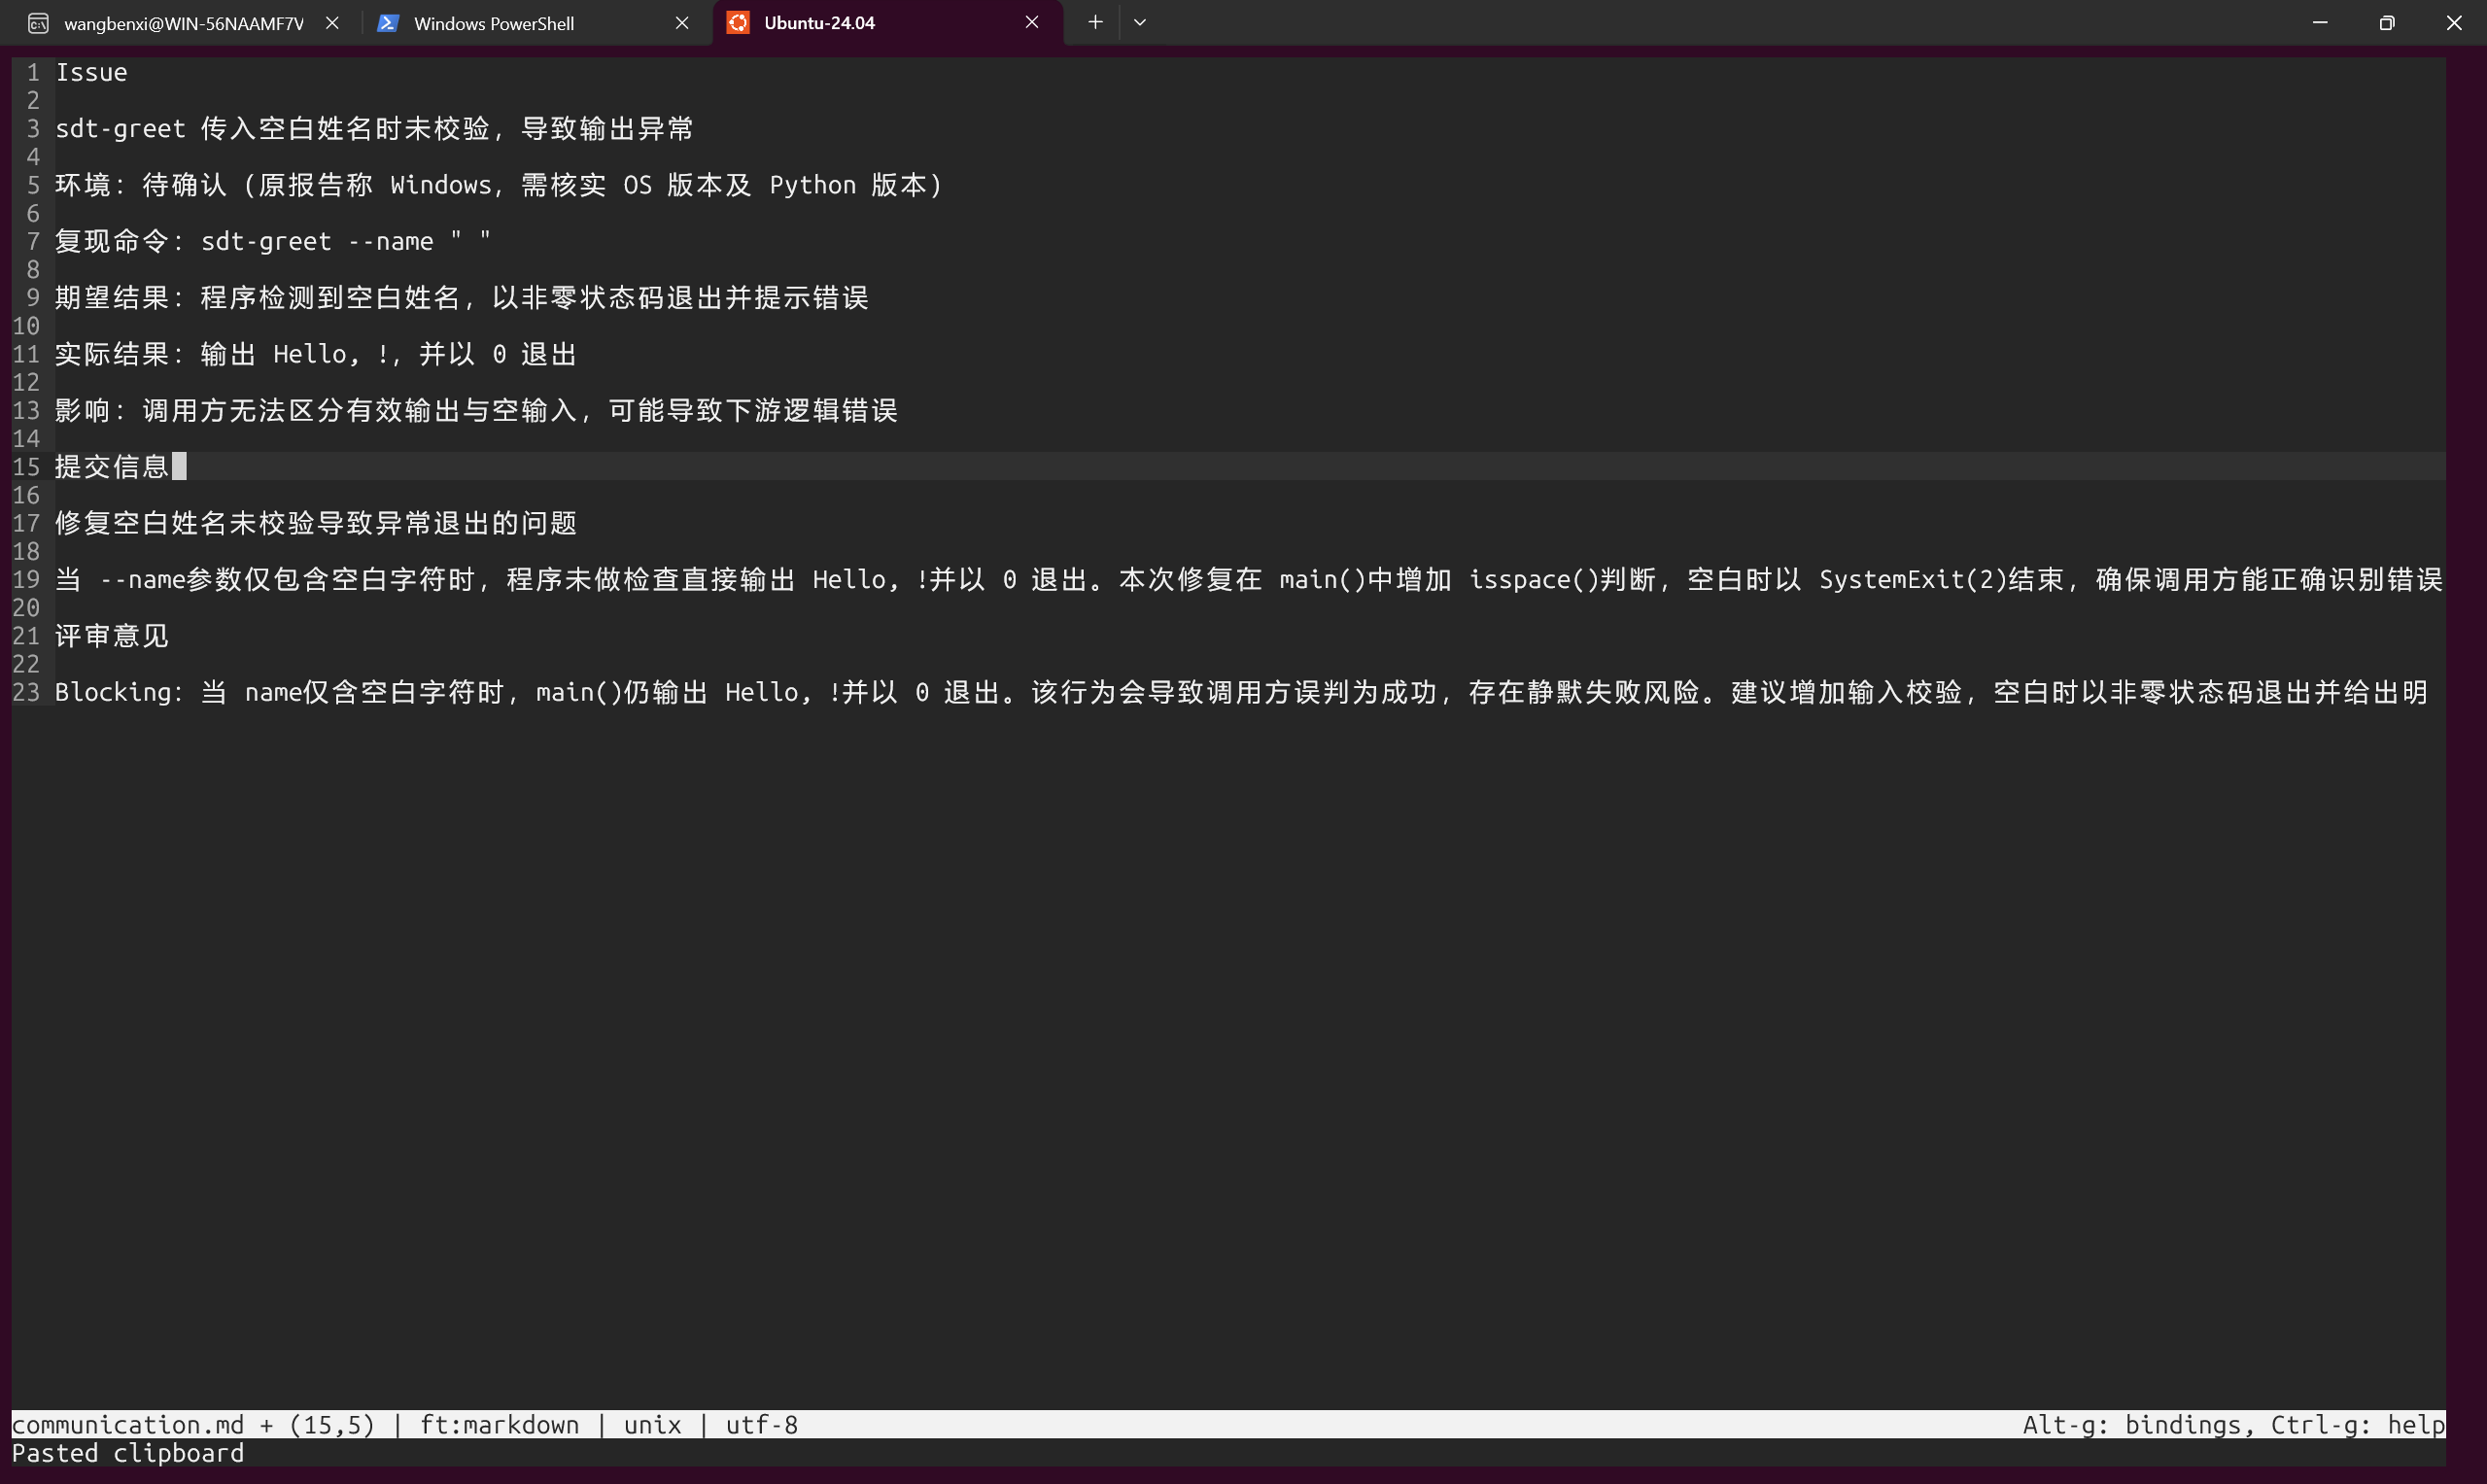
\includegraphics[width=0.98\textwidth]{q11-1.png}
  \caption{q11：可执行的协作材料——Issue、提交信息、评审意见}
  \label{fig:q11}
\end{figure}

\subsection{结果分析}

\begin{itemize}
  \item \textbf{Issue 改写}：
        标题从模糊的"运行不了"改为具体的"空白姓名未校验导致输出异常"；
        环境标注"待确认"，不臆测；
        提供可复制的复现命令 \texttt{sdt-greet --name "   "}；
        期望/实际结果清晰对比（非零退出 vs 输出 \texttt{Hello, !} 并以 0 退出）；
        增加影响描述，帮助评估优先级；
  \item \textbf{提交信息改写}：
        标题采用祈使语气"修复 \ldots 的问题"，而非"fix bug"；
        正文说明问题根因（未做检查直接输出）和解决方案（增加 \texttt{isspace()} 判断）；
        遵循 Git 提交信息约定：标题 $<$ 50 字符、正文 72 字符换行；
  \item \textbf{评审意见改写}：
        标注 \textbf{Blocking} 明确优先级；
        指出具体行为（name 仅含空白时 \texttt{main()} 仍输出并以 0 退出）；
        分析风险（调用方误判成功、静默失败）；
        给出建议动作（增加输入校验、非零退出码）；
  \item \textbf{字数控制}：全文约 380 字，符合 400 字以内的约束。
\end{itemize}

% ============================================================
\section{q12：修复一个可复现的线性回归训练循环}

\subsection{题目要求}

主题：Python 与 PyTorch。补全给定代码的两处 TODO，完成一次 PyTorch CPU 训练：
\begin{itemize}
  \item 补全训练循环，正确调用 \texttt{zero\_grad}、\texttt{backward} 和 \texttt{step}；
  \item 训练后调用 \texttt{model.eval()}，并在 \texttt{torch.no\_grad()} 中计算最终损失；
  \item 打印最终损失、weight 和 bias；最终损失应小于 0.001；
  \item 不得直接把 weight 和 bias 赋值为 3 和 $-1$。
\end{itemize}

\subsection{实验步骤}

给定代码中两处 TODO：
\begin{enumerate}
  \item 训练循环内：\texttt{opt.zero\_grad()} $\to$ \texttt{loss.backward()} $\to$ \texttt{opt.step()}；
  \item 训练结束后：\texttt{model.eval()} + \texttt{with torch.no\_grad():} 中计算并打印最终 loss、weight、bias。
\end{enumerate}

完整的 \texttt{train.py}：

\begin{lstlisting}[language=Python]
import torch
from torch import nn

torch.manual_seed(20260907)

x = torch.linspace(-1, 1, 101).reshape(-1, 1)
y = 3 * x - 1

model = nn.Linear(1, 1)
loss_fn = nn.MSELoss()
opt = torch.optim.SGD(model.parameters(), lr=0.1)

for _ in range(200):
    pred = model(x)
    loss = loss_fn(pred, y)
    opt.zero_grad()      # TODO 1: 清空梯度
    loss.backward()      # TODO 1: 反向传播
    opt.step()           # TODO 1: 更新参数

model.eval()             # TODO 2: 切换到评估模式
with torch.no_grad():    # TODO 2: 禁用梯度追踪
    final_loss = loss_fn(model(x), y)
    print(f"Final loss: {final_loss.item():.6f}")
    w, b = model.weight.item(), model.bias.item()
    print(f"Weight: {w:.6f}")
    print(f"Bias: {b:.6f}")
\end{lstlisting}

运行：

\begin{lstlisting}[language=bash]
cd q12
python3 -m venv venv && source venv/bin/activate
pip install torch --index-url https://download.pytorch.org/whl/cpu
python train.py
# Final loss: 0.000000
# Weight: 2.999997
# Bias: -1.000000
\end{lstlisting}

\subsection{运行结果与截图}

图~\ref{fig:q12} 展示了从创建 \texttt{q12/train.py} 到训练完成的全过程。

\begin{figure}[htbp]
  \centering
  \begin{subfigure}[b]{0.98\textwidth}
    \centering
    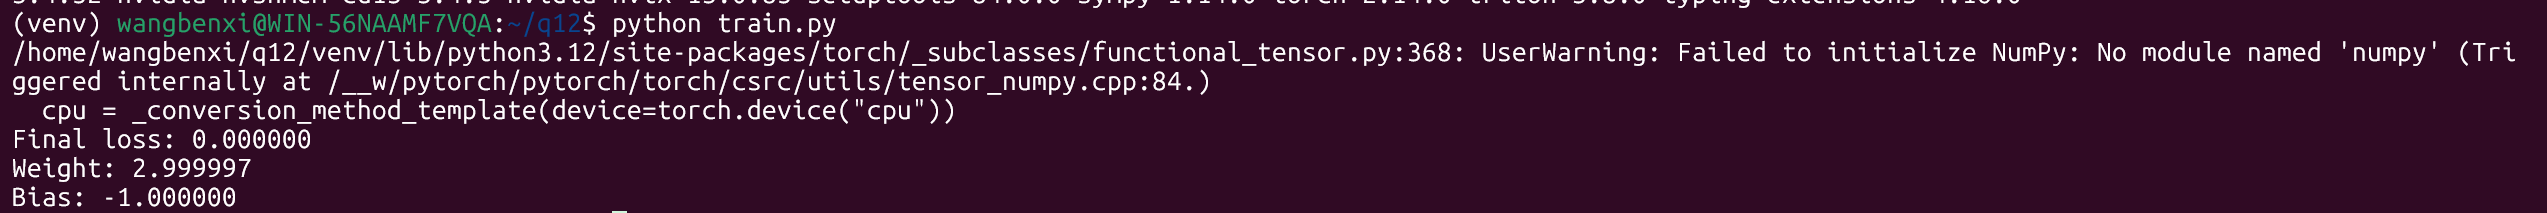
\includegraphics[width=\linewidth]{q12-1.png}
    \caption{\texttt{mkdir -p q12}、\texttt{micro q12/train.py}、\texttt{cd q12}、\texttt{python3 train.py}}
  \end{subfigure}

  \vspace{0.5em}
  \begin{subfigure}[b]{0.98\textwidth}
    \centering
    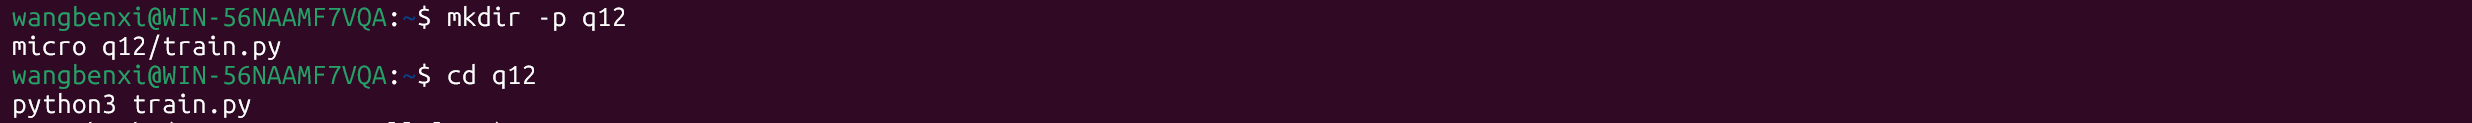
\includegraphics[width=\linewidth]{q12-2.png}
    \caption{训练输出：\texttt{Final loss: 0.000000}、\texttt{Weight: 2.999997}、\texttt{Bias: -1.000000}}
  \end{subfigure}
  \caption{q12：PyTorch 线性回归训练循环补全与验证}
  \label{fig:q12}
\end{figure}

\subsection{结果分析}

\begin{itemize}
  \item \textbf{训练循环补全}：每轮迭代依次执行
        \texttt{pred = model(x)}（前向传播）$\to$ \texttt{loss = loss\_fn(pred, y)}（计算损失）$\to$
        \texttt{opt.zero\_grad()}（清空上轮梯度）$\to$ \texttt{loss.backward()}（反向传播计算梯度）$\to$
        \texttt{opt.step()}（SGD 更新参数）；三行代码顺序不能交换，尤其 \texttt{zero\_grad}
        必须在 \texttt{backward} 之前；
  \item \textbf{eval / no\_grad}：训练 200 轮后调用 \texttt{model.eval()}
        切换到评估模式（关闭 Dropout、BatchNorm 等训练时特有的行为），
        再用 \texttt{with torch.no\_grad()} 禁用梯度追踪，
        减少内存分配并避免干扰评估；
  \item \textbf{收敛验证}：目标函数 $y = 3x - 1$，期望 weight$=$3、bias$=-1$；
        训练输出 Weight 2.999997、Bias $-1.000000$、Final loss 0.000000，
        符合 loss $< 0.001$ 的要求；固定随机种子 \texttt{torch.manual\_seed(20260907)}
        保证可复现；
  \item \textbf{注意事项}：PyTorch CPU 安装较慢，使用
        \texttt{--index-url https://download.pytorch.org/whl/cpu}
        直接从 PyTorch 官方 CPU 轮子安装，避免源码编译。
\end{itemize}

% ============================================================
\section{代码与仓库}

项目已托管至 GitHub：
\url{https://github.com/liangbaikai-666/tool-25020007117}

\subsection{Git 提交记录}

\texttt{git log --all --graph --decorate --oneline} 输出如下
（本次作业以八个提交推送至 \texttt{origin/main}）：

\begin{lstlisting}[language=bash, numbers=none]
* 4d10f5e (HEAD -> main) 第三次作业: report3.pdf 编译产物
* dab5537 第三次作业: q09-q12 实验截图
* bd3537f 第三次作业: report3.tex 实验报告
* 1d4d1d3 第三次作业: q12 PyTorch线性回归训练
* c804adb 第三次作业: q11 协作材料改写 - Issue/提交信息/评审意见
* 4a05b9d 第三次作业: q10 清理嵌套目录
* 6a84240 第三次作业: q10 AI驱动修复循环 - 空白姓名SystemExit(2)
* d6a240d 第三次作业: q09 包结构与源码
\end{lstlisting}

提交 \texttt{d6a240d} 包含 q09 的包结构源码；
\texttt{6a84240}+\texttt{4a05b9d} 包含 q10 的测试、修复后 \texttt{cli.py} 和 \texttt{ai\_log.md}
（第二个提交清理了复制 q09 时误带入的嵌套目录）；
\texttt{c804adb} 包含 q11 的 \texttt{communication.md}；
\texttt{1d4d1d3} 包含 q12 的 \texttt{train.py}；
\texttt{bd3537f} 包含实验报告 \texttt{report3.tex}；
\texttt{dab5537} 包含 q09--q12 的实验截图；
\texttt{4d10f5e} 包含 \LaTeX{} 编译产物 \texttt{report3.pdf}。

% ============================================================
\section{结论}

通过本次实验，完成了四道课上实验题，主要收获如下：

\begin{itemize}
  \item \textbf{Python 包构建与 wheel 安装（q09）}：掌握了
        \texttt{pyproject.toml} 定义包元数据、\texttt{python -m build}
        构建 sdist + wheel、干净虚拟环境从 wheel 安装验证的完整流程；
        \texttt{[project.scripts]} 声明命令行入口点，
        \texttt{[tool.setuptools.packages.find]} 处理 src-layout 的包定位；
  \item \textbf{测试驱动 + 智能体协作（q10）}：实践了
        "写失败测试 $\to$ 让智能体修改 $\to$ 验证通过 $\to$ 记录" 的闭环；
        发现 \texttt{ModuleNotFoundError} 是 src-layout 项目未以
        \texttt{pip install -e .} 可编辑安装的常见陷阱；
        \texttt{monkeypatch} + \texttt{pytest.raises} + \texttt{capsys}
        三件套完整模拟命令行参数并验证退出码；
  \item \textbf{可执行协作材料（q11）}：将三段模糊、不可复现的协作材料
        改写为可执行的 Issue（含复现命令、期望/实际对比、影响）、
        祈使语气的提交信息（标题 50 字符 + 正文 72 字符换行）、
        带 \textbf{Blocking} 优先级标注的评审意见（具体行为、风险、建议动作）；
  \item \textbf{PyTorch 训练循环（q12）}：补全了
        \texttt{zero\_grad} $\to$ \texttt{backward} $\to$ \texttt{step} 三行训练核心，
        以及 \texttt{eval} + \texttt{no\_grad} 评估模式；
        200 轮 SGD 训练线性回归，weight 2.999997 $\approx$ 3、
        bias $-1.000000 \approx -1$、loss 0.000000 $<$ 0.001，收敛验证通过。
\end{itemize}

总体而言，本实验覆盖了"打包发布 $\to$ 智能体协作 $\to$ 沟通表达 $\to$ 深度学习"
四个开发工具主题：从把代码封装成可分发的 wheel，到借助智能体完成测试驱动修复，
再到将协作材料写成工程师能直接执行的格式，最后用 PyTorch 实现简单的线性回归训练。
全部代码、截图与报告已提交至 GitHub
（commits \texttt{d6a240d}--\texttt{1d4d1d3}，\texttt{origin/main}）。

\end{document}
